\documentclass{article}

\usepackage{amsmath}
\usepackage{amssymb}
\usepackage{amsfonts}
\usepackage{mathtools}

\usepackage[thmmarks, amsmath]{ntheorem}

\usepackage{graphicx}
\usepackage{float}

\usepackage{diffcoeff}
\diffdef{}{op-symbol=\mathrm{d},op-order-sep=0mu}

\usepackage{cancel}
\usepackage{interval}

\usepackage{enumitem}

\setlist[enumerate,1]{label=(\alph*)}

\title{Algebraic Topology Homework 1}
\author{Duarte Maia}
%\date{}

\theoremstyle{plain}
\theorembodyfont{\upshape}
\theoremseparator{.}
\newtheorem{theorem}{Theorem}
\newtheorem{prop}{Prop}
\renewtheorem*{prop*}{Prop}
\newtheorem{lemma}{Lemma}
\newtheorem*{ex}{Exercise}

\theoremstyle{nonumberplain}
\theoremheaderfont{\itshape}
\theorembodyfont{\upshape}
\theoremseparator{:}
\theoremsymbol{\ensuremath{\blacksquare}}
\newtheorem{proof}{Proof}
\newtheorem{sol}{Solution}

\theoremsymbol{\text{\textit{(End proof of lemma)}}}
\newtheorem{lemmaproof}{Proof of lemma}

\newcommand{\R}{\mathbb{R}}
\newcommand{\C}{\mathbb{C}}
\newcommand{\Z}{\mathbb{Z}}
\newcommand{\Q}{\mathbb{Q}}

\newcommand{\kk}{\Bbbk}

\newcommand{\PP}{\mathbb{P}}
\newcommand{\FF}{\mathcal{F}}

\newcommand{\I}{\mathrm{i}}
\newcommand{\e}{\mathrm{e}}

\newcommand{\id}{\mathrm{id}}

\newcommand{\conj}[1]{\overline{#1}}

\DeclareMathOperator{\inte}{int}
\DeclareMathOperator{\codim}{codim}
\newcommand{\grad}{\nabla}


\DeclareMathOperator{\spec}{spec}

\DeclarePairedDelimiter{\abs}{\lvert}{\rvert}
\DeclarePairedDelimiter{\norm}{\lvert}{\rvert}
\DeclarePairedDelimiter{\Norm}{\lVert}{\rVert}
\DeclarePairedDelimiter{\braket}{\langle}{\rangle}


\begin{document}
\maketitle

\begin{ex}[0:4]
Show that if $A$ is a weak deformation retract of $X$ then $A$ and $X$ are homotopically equivalent.
\end{ex}

\begin{sol}
Let $F \colon X \times I \to X$ be the weak deformation retract. Set $f \colon A \to X$ as the inclusion, and $g \colon X \to A$ as $F_1$. We claim that $f \circ g$ and $g \circ f$ are homotopic to the identities in $X$ and $A$ respectively.

We begin by noting that, by definition, $F$ is a homotopy between the identity on $X$ and $g = f \circ g$. Then, notice that $F$ restricts to a function $A \times I \to A$, and this restriction is a homotopy between the identity on $A$ and $g|_A = g \circ f$. This completes the proof.
\end{sol}

\begin{ex}[0:6]
\leavevmode
\begin{enumerate}
\item Show that $X$ deformation retracts to any point in $[0,1] \times \{0\}$ but not any other point.

\item Show that $Y$ is contractible but does not deformation retract onto any point.

\item Show that there is a weak deformation retract of $Y$ onto $Z$, but no true deformation retraction.
\end{enumerate}
\end{ex}

\begin{sol}
\leavevmode
\begin{enumerate}
\item To show that $X$ deformation retracts to any point $(x,0)$ is easy: $X$ deformation retracts to $[0,1] \times \{0\}$ through $F((x,y),t) = (x,(1-t)y)$, which in turn deformation retracts to any of its elements by a straight-line homotopy.

Now, suppose $F \colon X \times I \to X$ is a deformation retract of $X$ into some point $(x_0,y_0) \in X$, with $y_0 > 0$. Note that, for each point $(x,y)$ with $x \neq x_0$, the path traced by $F_t(x,y)$ as $t$ goes from $0$ to $1$ must at some point pass through $[0,1] \times \{0\}$. This is by Bolzano's theorem, as the first coordinate of $F_t(x,y)$ is varying between two distinct numbers, and must therefore be irrational for some $t \in [0,1]$, and if $(x',y') \in X$ with $x'$ irrational then $y'$ must be $0$.

Still assuming that $F$ exists, pick a sequence $(x_n, y_n) \in X$ which converges to $(x_0, y_0)$, with all $x_n$ distinct from $x_0$. (For example, set $y_n = y_0 - \frac1n$, $x_n = x_0 + \frac1n$; this is in $X$ for $n$ big enough.) As per the previous paragraph, for each $n$ pick some $t_n \in [0,1]$ such that $F_{t_n}(x_n,y_n) \in [0,1] \times \{0\}$, and taking a sublimit if necessary we may assume that $t_n$ converges to some $t \in [0,1]$. Now, by continuity, we must have
\begin{equation}
\lim_n F_{t_n}(x_n,y_n) = F_t(x_0,y_0) = (x_0,y_0).
\end{equation}

However, this is impossible because the second coordinate of $F_{t_n}(x_n,y_n)$ is always null, while $y_0 > 0$. This is a contradiction, which proves that $F$ cannot exist.

\item To show that $Y$ is contractible, we begin by solving (c) (see below). Since $Z$ is contractible (it is homeomorphic to the real line), it is possible to find a homotopy between $\id_Y$ and a constant map by: for $t \in [0,\frac12]$, do the weak deformation of $Y$ to $Z$, and for $t \in [\frac12,1]$ compose it with a retraction of $Z$ to a point.

To show that $Y$ is does not deformation retract onto any point, we show that if such a thing happened then we would have a contradiction with (a).

Suppose $Y$ deformation retracts to $p$. Then, $p$ will be in one of the copies of $X$. If $p \in Z$, it is actually in two copies of $X$; choose the one in which $p$ is in the `comb-y area', and not in the base.

Now, we claim that there is a retraction of $Y$ to this copy of $X$. It may be built explicitly as follows. Consider the infinite horizontal strip in which $Y$ is contained (actually the closure of $Y$). Within this strip, consider the triangle in which $X$ is contained (the closure of $X$). Then, there is a retraction of this rectangle onto this triangle, given by horizontal projection. Next, it suffices to show (and it is obvious) that this retraction, when restricted to $Y$, has image in $X$, and therefore is a retraction of $Y$ to $X$.

Now, if $Y$ deformation retracted to $p$, by composing this deformation with the retraction outlined in the previous paragraph, we would obtain a deformation retraction of $X$ to $p$, which contradicts (a). The proof of (this part of) (b) is complete.

\item To solve this exercise, we take advantage of the following fact: the copies of $X$ in $Y$ are mostly independent from one another. More specifically, to check continuity of a map $Y \times I \to Y$ it suffices to verify that its restriction to $X_n \times I$ is continuous, where $X_n$ is any of the copies of $X$ that make up $Y$. This is trivially true by the pasting lemma, as the union all of these spaces makes up $X$ and each of them individually is closed in $X$.

Now, we will define an auxilliary map $F \colon X \times \R \to X$ by defining it on each $X_n \times \R$ as follows. In the sequence, assume that the $X_n$ are ordered left to right, so $X_{n+1}$ is directly to the right of $X_n$.

\begin{itemize}
\item For all $t \in \linterval{-\infty}{n-1}$, let $F_t$ be the identity on $X_n$. Then, for $t \in [n-\frac12,n]$, let $F_t$ be the linear retraction of $X_n$ onto its base.

\item Then, we let $F_{n+\frac12}$ be the vertical projection of $X_n$ onto $X_n \cap Z$, with $F_t$ interpolating continuously between $F_n$ and $F_{n+\frac12}$ by moving the points through $Z$. To be more explicit, any point $x \in X_n$ has its trajectory going as follows: first, follow the `hairs' to the base of $X_n$, then move to the left along $Z$ to the vertical projection of $x$ on $Z$.

\item From hereon out it gets kind of complicated to explain with words, so just see the following picture. At each step we show the image of four segments in $X_n$ as they travel through $X$, colored in red, green, blue and dark blue. The gray `ghost $X$' is just there as a referential. In the second row, we have a copy of this picture but reflected vertically; it represents what this deformation does to $X_{n+1}$. It is juxtaposed with what it does to $X_n$ so that it is clear that the motions are compatible, i.e. the restriction to $X_n \cap X_{n+1}$ is well-defined.

\begin{figure}[H]
\centering
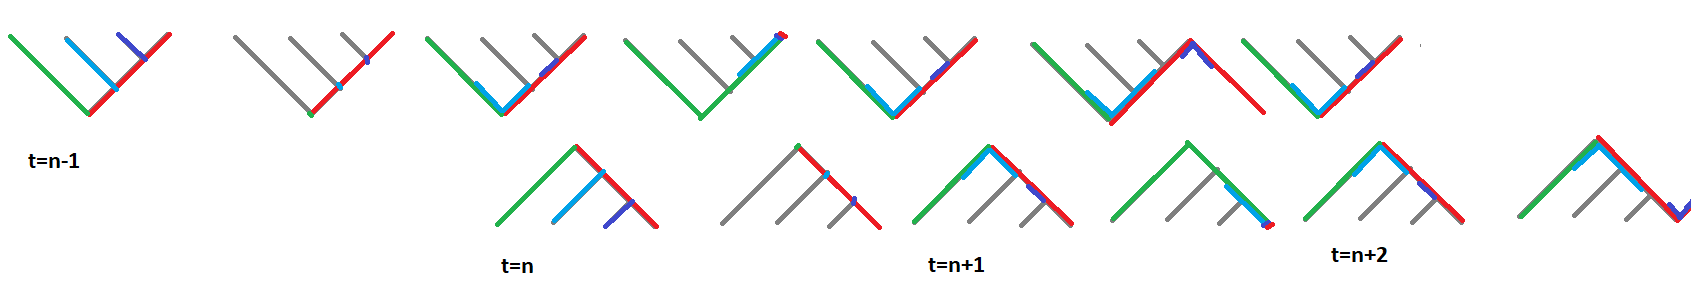
\includegraphics[width=\linewidth]{combs}
\end{figure}

\item Anyway, for $t > n+2$, $F_t$ does not move anymore.
\end{itemize}

So this complicated function which I just described is a function $F \colon X \times \R \to X$. It can be extended to $X \times [-\infty, \infty]$, because from the perspective of each $X_n \times \R$ it does not move before or past a certain point, so it can be extended to $-\infty$ as the identity and to $+\infty$ as the vertical projection on $Z$. Since $[-\infty, \infty] \cong I$, we have a homotopy of maps. The first one is $F_{-\infty}$, which is the identity. The second is $F_{+\infty}$, which is the vertical projection on $Z$. Moreover, note that in the description of $F$ above, a point which starts on $Z$ never leaves $Z$, so $F$ is a weak deformation retraction.

\medskip

Now, let us show that $Z$ cannot be a strong deformation retraction of $Y$. As in (b), if there were, we could compose this deformation retraction with a retraction of $Y$ onto (any copy of) $X$, in order to obtain a strong deformation retraction of $X$ onto $[0,1] \times \{0\} \cup \{0\} \times [0,1]$. This subset of $X$, in turn, can be retracted by deformation to $(0,1)$, and composing these two motions we would have a deformation retraction of $X$ to a point not in the base, which is impossible. This completes the proof.
\end{enumerate}
\end{sol}

\begin{ex}[0:16]
Show that $S^\infty$ is contractible.
\end{ex}

\begin{sol}
We recall that Hatcher's definition of $S^\infty$ is as follows: if we see each $S^n$ as included in $S^{n+1}$ (say, as being the equator), we let $S^\infty = \bigcup_n S^n$ endowed with the weak topology. However, we may also see it as $\bigcup_n D^n$, where $D^n$ is the $n$-dimensional closed disk, which is seen as a subset of $S^n$, e.g. by taking one of the hemispheres. Under this perspective, $S^\infty$ is also endowed with the weak topology; we will now prove this claim.

If $U \subseteq S^\infty$ is open, then for any $n$ we have $U \cap S^n$ is an open subset of $S^n$. As a consequence, $U \cap D^n$ is also an open subset of $D^n$ by definition of the subspace topology. Therefore, a weakly open set in $\bigcup S^n$ is also weakly open in $\bigcup D^n$ (where the $D^n$ are included in each other as hemispheres). On the other hand, a similar argument holds if we see $S^n$ as a subspace of $D^{n+1}$, so in truth the two topologies coincide.

To proceed, notice that each $D^n$ is a deformation retract of $D^{n+1}$ (straight-line homotopy between the identity and the projection through the last axis). The result then follows from the following lemma.

\begin{lemma}
Let $X_1 \subseteq X_2 \subseteq \dots$ be a sequence of topological spaces whose topologies are compatible (i.e. the topology of $X_n$ is the subspace topology in subsequent spaces), and let $X = \bigcup X_n$ be their union endowed with the weak topology. Suppose moreover that every $X_n$ is a deformation retraction of $X_{n+1}$. Then, $X_1$ is a deformation retraction of $X$.
\end{lemma}

\begin{lemmaproof}
We will need some machinery to prove this lemma. First, we remark that the topology on $X$ is the colimit topology from the diagram $X_1 \hookrightarrow X_2 \hookrightarrow \dots$, so that a function on $X$ is continuous iff its restriction to each $X_n$ is continuous. This is easy to prove directly.

Next, we require a fact about path homotopies: a homotopy $F \colon X \times I \to X$ is the same as a continuous map $f \colon X \to X^I$, where $X^I$ is the space of paths in $X$ endowed with the compact-open topology. This fact, as well as the definition of compact-open topology, can be found around page 530 of Hatcher. In particular, we are using parts (b) and (c) of proposition A.14.

This fact allows us to use the universal property of the colimit on $X$ to claim the following: if $F \colon X \times I \to X$ restricts to a continuous map on every $X_n \times I \to X$, then $F$ itself is continuous. (The proof is obvious. $F$ is the same as a continuous map $X \to X^I$, which is continuous iff all its restrictions to $X_n$ are, and those correspond to restrictions of $F$ to $X_n \times I$.)

Now, let $F^n$ be the deformation retraction from $X_{n+1}$ to $X_n$. We define $F \colon X \times I \to X$ as follows: given $x \in X_n$, $F_t(x)$ stays still for $t \in [0,2^{-n}]$. Then, for $t \in [2^{-n}, 2^{-n+1}]$ it equals $F^{n-1}_{2^n t - 1}(x)$. Note that then $y = F_{2^{-n+1}}(x) \in X_{n-1}$, so that for $t \in [2^{-n+1}, 2^{-n+2}]$ we may set $F_t(x) = F^{n-2}_{2^{n-1} t - 1}(y)$, and so on recursively until $n = 1$.

To show that $F$ is continuous, we show that it is continuous on $X_n \times I$. To this effect, note that its restriction to $X_n \times I$ is given by:
\begin{itemize}
\item $F_t$ is the identity for $t \leq 2^{-n}$,
\item $F_t$ coincides with $F^{n-1}_{2^n t - 1}$ for $2^{-n} \leq t \leq 2^{-n+1}$,
\item $F_t$ coincides with $F^{n-2}_{2^{n-1} t - 1} \circ F^{n-1}_1$ for $2^{-n+1} \leq t \leq 2^{-n+2}$,
\item And so on, until $F_1$ is a retraction to $X^1$ (because it is the composition of a retraction of $X^n$ to $X^{n-1}$, a retraction from $X^{n-1}$ to $X^{n-2}$, and so on).
\end{itemize}

Evidently $F$ is continuous on $X_n \times I$ by the pasting lemma, and so by the claim above it is continuous on $X \times I$. Moreover, it preserves $X^1$ fixed because each $F^n$ does, and for all $x \in X$ we have $F_1(x) \in X$ by construction.
\end{lemmaproof}

This completes the solution of the exercise.
\end{sol}

\begin{ex}[0:20]
Show that the self-intersecting Klein bottle is homotopy equivalent to $S^1 \wedge S^1 \wedge S^2$.
\end{ex}

\begin{sol}
Proof by pictures. In the following figure, each step consists of collapsing or uncollapsing some contractible subcomplex of the Klein bottle with an appropriately chosen CW structure. Thus, each step is a homotopy equivalence by propositions 0.17 and 0.16 of Hatcher. The figure should be read left to right.

\begin{figure}[H]
\centering
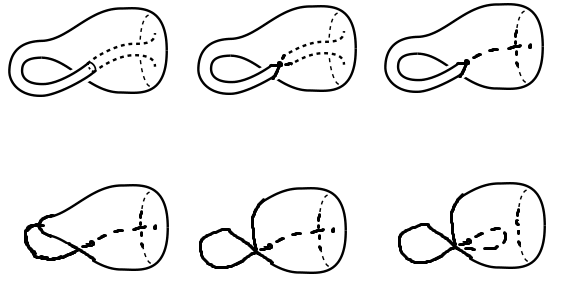
\includegraphics{klein}
\end{figure}

The end state is evidently $S^1 \wedge S^1 \wedge S^2$.
\end{sol}

\begin{ex}[0:23]
Show that a CW complex is contractible if it is the union of two contractible subcomplexes whose intersection is also contractible.
\end{ex}

\begin{sol}
Let $A$ and $B$ be the subcomplexes in question. Then, by propositions 0.17 and 0.16 of Hatcher, $A \cup B$ is homotopy equivalent to $(A \cup B)/A$. This in turn is homeomorphic to $B/(A \cap B)$,\footnote{This is readily seen because the corresponding CW complexes are the same.} which is equivalent to $B$ by the same propositions, and likewise $B$ is equivalent to $B/B = *$. This concludes the proof.
\end{sol}

\begin{ex}[1.1:6]
Show that $\Phi \colon \pi(X,x_0) \to [S^1, X]$ is surjective if $X$ is path-connected and that $\Phi([f]) = \Phi([g])$ iff $f$ and $g$ are conjugate to each other.
\end{ex}

\begin{sol}
First, suppose that $X$ is path-connected, and let $\eta \colon S^1 \to X$. We will show that there exists some $[f] \in \pi(X,x_0)$ with $\Phi([f])$ homotopic to $\eta$.

To this effect, pick some point $p \in S^1$ and construct $f \colon [0,1] \to X$ in the following manner: For $t \in [0,\frac13]$ go from $x_0$ to $\eta(p)$. Then, for $t \in [\frac13,\frac23]$, follow along $\eta$ (identifying $S^1$ with $[\frac13,\frac23]$ mod endpoints, with the endpoints being equal to $p$), and then for $t \in [\frac23,1]$ go from $\eta(p)$ back to $x_0$, following the opposite path as before.

Evidently, $[f] \in \pi(X,x_0)$. Moreover, $\Phi([f])$ is a map from $S^1 \to X$ which is homotopic to $\eta$, because it is built from $\eta$ by adding a section which does a thing and then undoes it. This proves surjectiveness.

\smallskip

Now, suppose that $\Phi([f]) = \Phi([g])$. Then, there is a homotopy $H$ between (the obvious representatives of) $\Phi([f])$ and $\Phi([g])$.

Now, by definition, $f(t) = H_0(\e^{\I t})$. Moreover, by stretching the square in an appropriate way, $H$ provides a path homotopy between $f(t)$ and the composition of the paths: $H_t(1)$, $H_1(\e^{\I t})$, $H_{1-t}(1)$. The middle path is evidently $g$, and the other two paths are inverses to each other (say $\gamma$ and $\gamma^{-1}$), so we conclude
\begin{equation}
f \simeq \gamma g \gamma^{-1}.
\end{equation}

Since $\gamma \in \pi(X,x_0)$, $[f]$ and $[g]$ are conjugates to each other.
\end{sol}

\begin{ex}[1.1:13]
Show that $i_* \colon \pi(A,x_0) \to \pi(X,x_0)$ is surjective iff every path in $X$ with endpoints in $A$ is path-homotopic to a path in $A$.
\end{ex}

\begin{sol} (In the following, $[f]$ denotes the homotopy class of $f$ in $X$ and $[g]_A$ denotes the homotopy class of $g$ in $A$.)
\begin{itemize}
\item ($\rightarrow$) Given a path $f$ in $X$ (with endpoints at $x_0$), its homotopy class is in the image of $\pi(A,x_0)$, so that there exists a path $[g]_A \in \pi(A,x_0)$ whose $X$-homotopy class is the same as that of $f$. In other words, $g$ is homotopic to $f$, and so is the path in $A$ that we sought.

\item ($\leftarrow$) Given arbitrary $[f] \in \pi(X,x_0)$, let $g$ be a path in $A$ to which $f$ is path-homotopic. Then, $i_*([g]_A) = [g] = [f]$. Hence, $i_*$ is surjective.
\end{itemize}
\end{sol}

\begin{ex}[1.1:20]
Let $f \colon X \times I \to X$ be a homotopy between the identity map and itself. Show that given $x_0$, the (homtopy class of the) path $f_t(x_0)$ is in the center of $\pi(X,x_0)$.
\end{ex}

\begin{sol}
Apply lemma 1.19 of Hatcher to $\Phi = f$. Taking into account that $f_1 = f_0 = \id_X$, this lemma tells us that conjugation by $h(t) = f_t(x_0)$ is the identity map. In other word, $h(t)$ commutes with everything and is hence in the center of $\pi(X,x_0)$.
\end{sol}

\end{document}